%% 
%% Copyright 2019 Elsevier Ltd
%% 
%% This file is part of the 'CAS Bundle'.
%% --------------------------------------
%% 
%% It may be distributed under the conditions of the LaTeX Project Public
%% License, either version 1.2 of this license or (at your option) any
%% later version.  The latest version of this license is in
%%    http://www.latex-project.org/lppl.txt
%% and version 1.2 or later is part of all distributions of LaTeX
%% version 1999/12/01 or later.
%% 
%% The list of all files belonging to the 'CAS Bundle' is
%% given in the file `manifest.txt'.
%% 
%% Template article for cas-dc documentclass for 
%% double column output.

%\documentclass[a4paper,fleqn,longmktitle]{cas-dc}
\documentclass[a4paper,fleqn]{cas-dc}

%\usepackage[authoryear,longnamesfirst]{natbib}
%\usepackage[authoryear]{natbib}
\usepackage[numbers]{natbib}
\usepackage{amsmath}



\usepackage{algorithm2e}
\usepackage[noend]{algcompatible}

\newcommand{\algorithmicinput}{\textbf{input}}

\newcommand{\INPUT}{\item[\algorithmicinput]}



\usepackage{textcomp}
\usepackage{graphicx}
\usepackage{caption}
\usepackage{siunitx}
%\usepackage{mathpazo}

\newcommand{\italicLt}{{it t}}

\begin{document}
\let\WriteBookmarks\relax
\def\floatpagepagefraction{1}
\def\textpagefraction{.001}
\shorttitle{Classification of Parkinson's disease patients using Bayesian deep learning based on fMRI data}
\shortauthors{Amin Amini, Mayam Amirmazlaghani}

\title [mode = title]{Classification of Parkinson's disease patients using Bayesian deep learning based on fMRI data}



\author[1]{Maryam Amirmazlaghani}
\cormark[1]
\ead{mazlaghani@aut.ac.ir}

\author[1]{Amin Amini}
\ead{amin-amini@aut.ac.ir}

\credit{Conceptualization of this study, Methodology, Software}

\address[1]{Department of Computer Engineering and Information Technology, Amirkabir University of Technology, Tehran, Iran}


\cortext[cor1]{Corresponding author}

\begin{abstract}
The goal of resting-state functional magnetic resonance imaging (fMRI) is to investigate the brain's functional connections by using the temporal similarity between blood oxygenation level-dependent (BOLD) signals in different regions of the brain “at rest” as an indicator of synchronous neural activity.
However having different images of patients' brains despite the sequential time-based information, may contain enough data to investigate their brains and enables us to recognize some diseases.
In this paper, we propose a novel method to automatically extract this non-time sequence-based information using a Bayesian deep learning algorithm based on a convolutional neural network (CNN).
Instead of using some predefined points of interest (POIs) we use the whole data in the training phase so those points of the brain which do not contain related information about the disease will be ignored automatically by the trained model.
Moreover, this method does not make any assumptions about the disease, patients, etc.,
makes it a possible universal disease diagnosis approach to differentiate diseases having an impact on brain functionality.
This method is a supervised algorithm with a small number of calculations using three-dimensional CNN.
Each fMRI scan (which contains {\it t} time slices of the brain) of patients will be divided into {\it t} different 3D images enabling us to make the dataset much bigger in number and calculations way simpler.
Subsequently, all of these images are fed to a Bayesian network similar to LeNet-5 (but in three dimensions) to train our model.
Then to determine if a person is suffering from Parkinson's or not, we test his/her {\it t} fMRI images and get {\it t} different results which leads to a fraction (probability) of how unhealthy his/her brain is and if that fraction is above 0.5 we can classify that sample as a Parkinson's patient.
\end{abstract}


%\begin{highlights}
%\item High accuracy with 
%\item Research highlights item 2
%\item Research highlights item 3
%\end{highlights}

\begin{keywords}
Functional magnetic resonance imaging (fMRI) \sep
Resting-state \sep
Disease diagnosis \sep
Bayesian deep learning \sep
Convolutional neural network (CNN) \sep
Parkinson's disease
\end{keywords}


\maketitle

\section{Introduction}

Intro





\section{Materials and methods}
\label{section:materials}





\subsection{Participants}
\label{section:participants}
We had 30 subjects with ACER over 85 and MMSE over 27, comprising 15 healthy controls \texttt{[HC, age 63.33 ± 5.25, 8 females ]}
and 15 patients diagnosed with Parkinson's disease  \texttt{[PD, age 70.73 ± 4.80, 8 females ]}.
Significant differences in age and ACER aong two groups were found \texttt{(age: p=0.0012 , ACER: p=0.015)}. However no significant difference in MMSE were found \texttt{(MMSE: p=0.315)}.

\subsection{Data acquisition}
\label{section:data}
fMRI scans were obtained from the OpenfMRI project which was acquired on a 3T Siemens Verio with repetition time (TR) = 2.5 s, echo time (TE) = 30ms, flip angle = 80°. Each sample contains 198 slices of $39 \times 64 \times 64$ voxels from the brains of patients. Subjects were instructed to close their eyes and to rest quietly during the scan session \cite{OpenFmri}.

\subsection{Data pre-processing}
\label{section:preprocessing}
The fMRI data were pre-processed using the standard modules of FMRIB Software Library v5.0 \cite{FMRIB}. The pre-processing steps for the anatomical data involved motion correction (MCFLRIT), skull stripping, and spatial smoothing (Gaussian kernel of 5-mm FWHM). Low level noise was removed using a high-pass temporal filtering. The functional images were then aligned to the individual's high-resolution T1-weighted scans, which were subsequently registered to the Montreal Neurological Institute standard space (MNI152) using affine linear registration. and resampled at 2mm cubic voxels. The product of the preprocessing step was used in the experiments.



\subsection{Three dimensional convolutional neural networks}
\label{section:3dCnn}
3D Convolutional Neural Networks which are inspired by human visual system are similar to classic neural networks. This architecture has been particularly designed based on the explicit assumption that raw data are three-dimensional that enables us to encode certain properties and also to reduce the amount of hyper parameters. The CNN topology utilizes spatial relationships to reduce the number of parameters which must be learned and thus improves upon general feed-forward back propagation training. Equation \eqref{eq:CnnVal} shows how value of each voxel is calculated from previous layer based on a fixed kernel \texttt{(size = P$\times$Q$\times$R)} and a bias for \texttt{j}th feature in \texttt{i}th layers where v is value, f is the activation function and w is filter weight \cite{Ji2013}.

\begin{equation}
v^{ xyz }_{ ij } = \\
f(  \\
b_{ij} +  \\
\sum_m \\ 
\sum_{p=0}^{P_i-1} \\
\sum_{q=0}^{Q_i-1} \\
\sum_{r=0}^{R_i-1} \\
\; w^{pqr}_{ijm}  \\
\; v ^ { (x+p)(y+q)(z+r) }_{ (i-1)m } \\
) \label{eq:CnnVal} 
\end{equation}

Since fMRI images are 3D time series and our experiment tries to find out if images contain any useful information despite their sequences, three dimensional CNN can be used as our computational core. A simple 3D CNN can be seen in Figure \ref{fig:CnnSample}

\begin{figure*}
	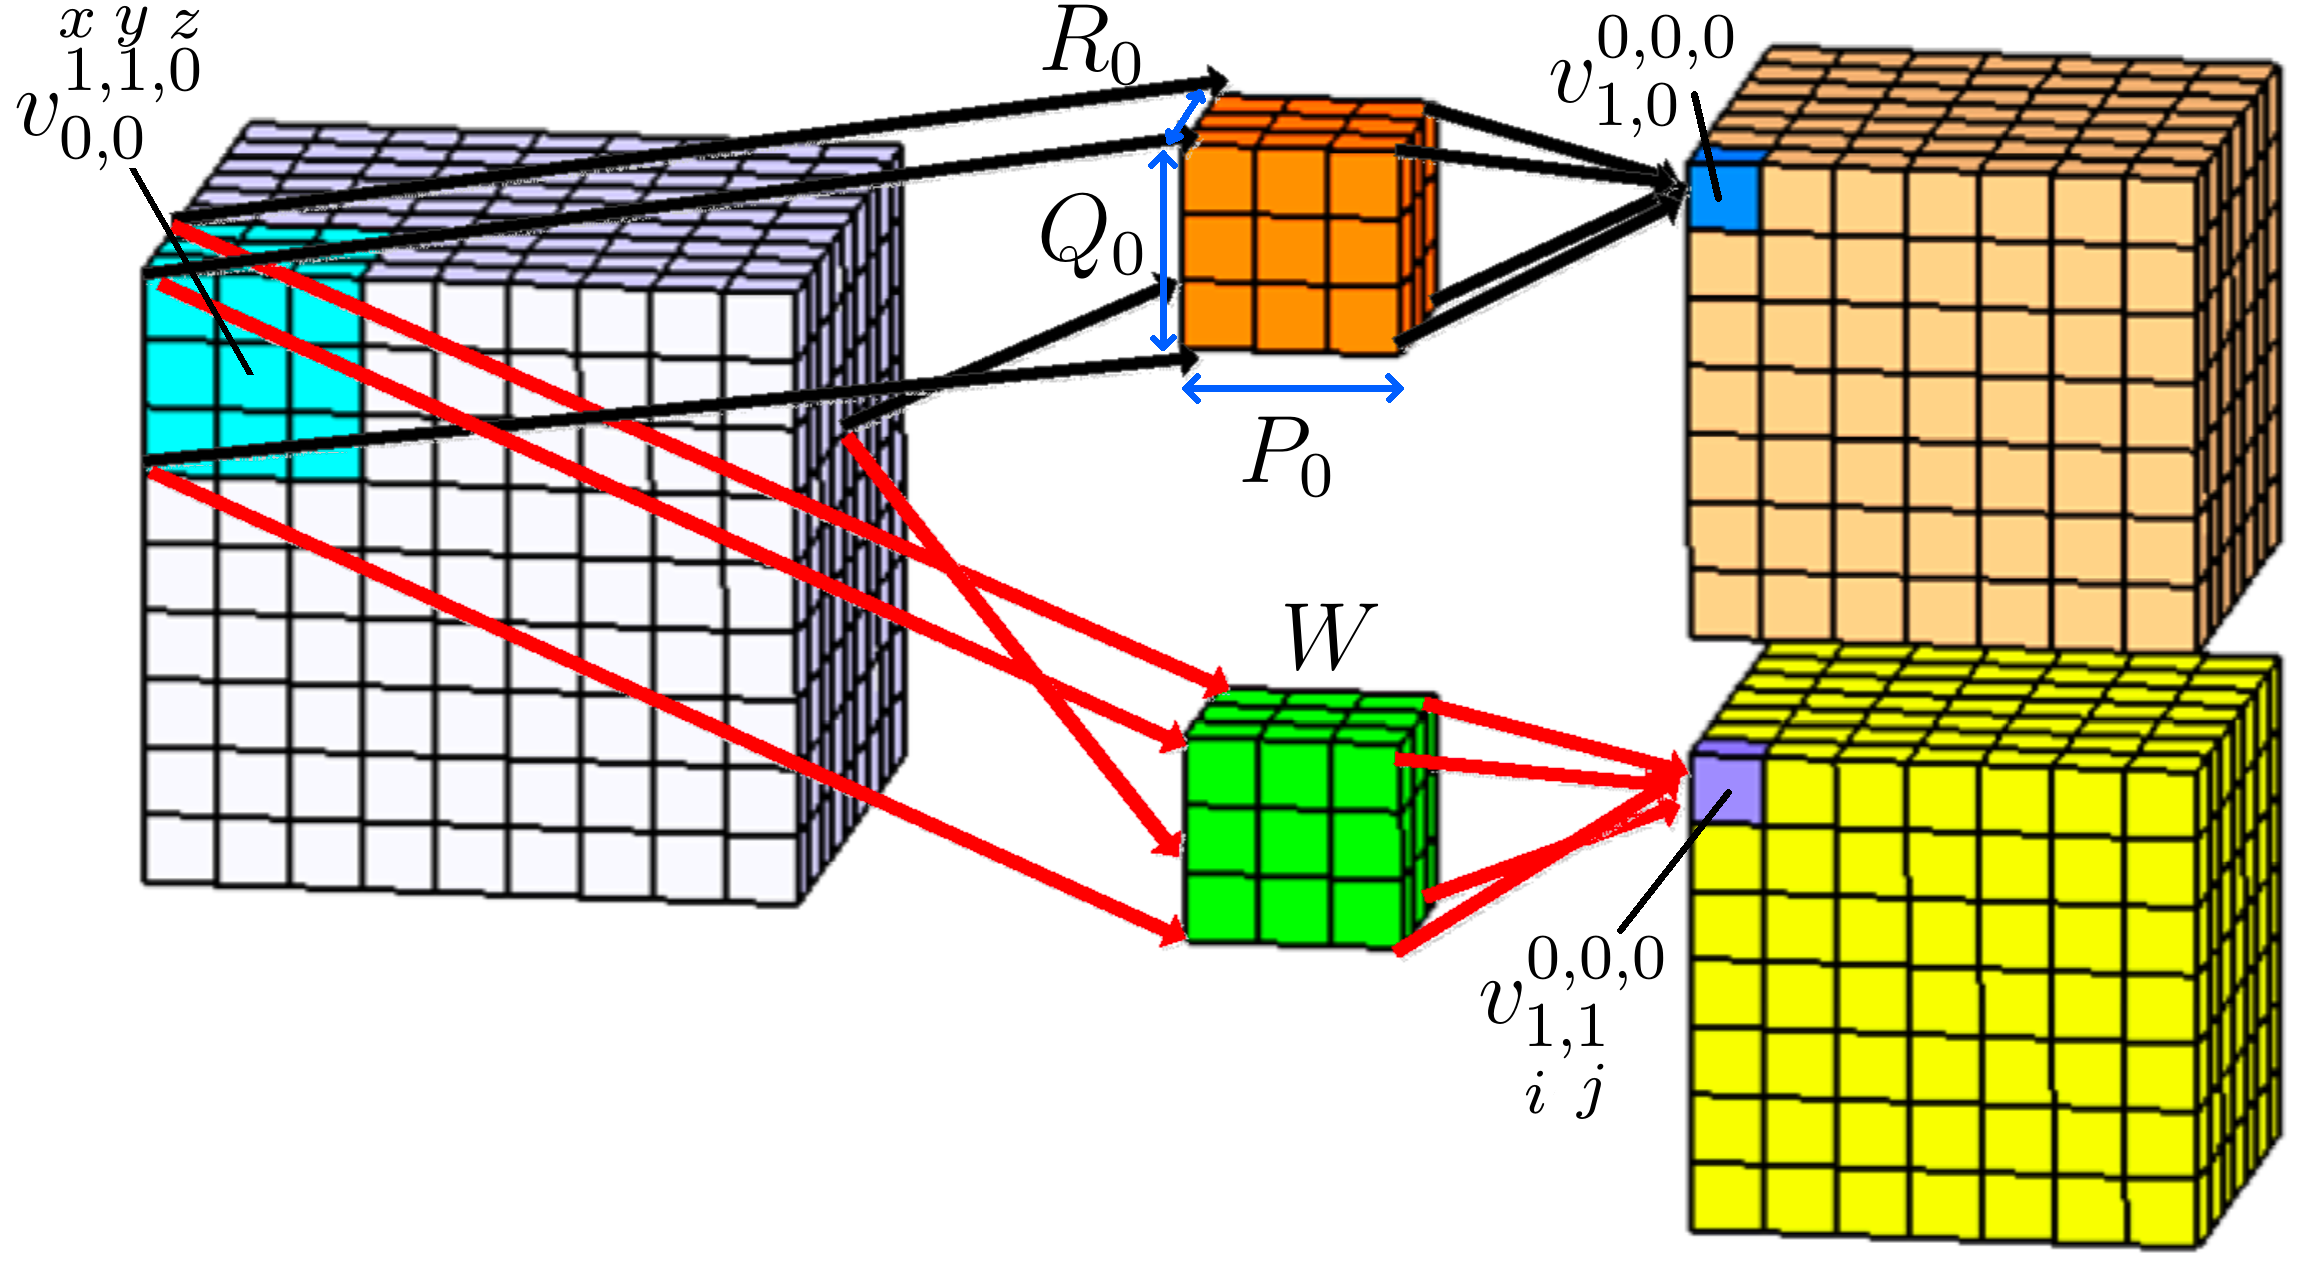
\includegraphics[width=0.8\linewidth]{images/3dCnn}
	\caption{3D CNN demonstration (kernel size = 3$\times$3$\times$3).}
	\label{fig:CnnSample}
\end{figure*}




\subsection{Bayesian deep learning}
\label{section:bayesianDL}
Deep learning has achieved significant success in many perception tasks including seeing (visual object recognition), reading (text understanding), and hearing (speech recognition). These are undoubtedly fundamental tasks for a functioning comprehensive artificial intelligence (AI) or data engineering (DE) system. However, in order to build a real AI/DE system, simply being able to see, read, and hear is far from enough. It should master
the ability of thinking.

Take medical diagnosis as an example. Besides seeing
visible symptoms (or medical images from MRI) and hearing descriptions from patients, a doctor has to look for relations among all the symptoms and preferably infer the corresponding etiology. Only after that can the doctor provide medical advice for the patients. In this example, although the abilities of seeing and hearing allow the doctor to acquire information from the patients, it is the thinking part that defines a doctor. Specifically, the ability of thinking here could involve causal inference, logic deduction, and dealing with uncertainty, which is apparently beyond the capability of conventional deep learning methods \cite{Wang2016}.

A neural network with arbitrary depth and non-linearities, with dropout applied before every weight layer, is mathematically equivalent to an approximation to the probabilistic deep Gaussian process \cite{Gal2016}.

Let $\hat{y}$ be the output of a NN model with $L$ layers and a loss function {\it E(·, ·)} such as the softmax loss or the Euclidean loss (square loss).We denote by $W_i$ the NN’s weight matrices of dimensions $K_i \times K_{i-1}$, and by $b_i$ the bias vectors of dimensions $K_i$ for each layer $i = 1, ..., L$. We denote by $y_i$ the observed output corresponding to input $x_i$ for $1 \leq i \leq N$ data points, and the input and output sets as $X, Y$. During NN optimization a regularization term is often added. We often use $L2$ regularization weighted by some weight decay $\lambda$, resulting in a minimization objective (often referred to as cost) and it can written as Equation  \eqref{eq:bayesianCnnDroupout} \cite{Gal2016}.

\begin{equation}
\mathcal{L}_{dropout} := 
    {1 \over N} \sum_{i=1}^{N} E(y_i , \hat{y_i}) + \\
    \lambda \sum_{i=1}^{L} ( \left|\left| W_i \right|\right|_2^2 + \left|\left| b_i \right|\right|_2^2 )
\label{eq:bayesianCnnDroupout} 
\end{equation}

Now of if we add dropout to the calculations each unit may remain the same with probability $p_i$ or dropped out (its value is set to zero). We use the same values in the backward pass propagating the derivatives to the parameters. Assume we are given a covariance function of the form of Equation \eqref{eq:nnCovariance}.

\begin{equation}
K(x, y) = \int p(w)p(b) \sigma (w^T x + b) \sigma (w^T y + b) dw db
\label{eq:nnCovariance}
\end{equation}

with some element-wise non-linearity {\it $\sigma$(·)} and distributions $p(w), p(b)$. It had been shown that a deep Gaussian process with L layers and covariance function $K(x,y)$ can be approximated by placing a variational distribution over each component of a spectral decomposition of the GPs’ covariance functions.

Let $W_i$ be a random matrix of dimensions $K \times K_{i-1}$ for each layer $i$, and write
$\omega = \{ W_i \}^L_{i=1}$. A priori,we let each row of $W_i$ distribute according to the $p(W)$ above. In addition, assume vectors $m_i$ of dimensions $K_i$ for each GP layer. The predictive probability of the deep GP model given some precision parameter $\tau > 0$ can be parameterized as Equation \eqref{eq:gpPriority}.

\begin{eqnarray}
\label{eq:gpPriority}
p(y | x,X,Y) = \int p(y|x,\omega) p(\omega|X,Y)d\omega \\ 
p(y|x,\omega) = \mathcal{N} (y ; \hat{y} (x,\omega) , \tau^{-1} I_D )  \nonumber \\
\hat{y} (x, \omega = \{ W_1, ..., W_L \}) =  \nonumber \\
\sqrt{1 \over K_L} W_L \sigma( ...  \sqrt{1 \over K_1} W_2 \sigma( W_1 x + m_1 ) ... )  \nonumber
\end{eqnarray}

The posterior distribution $p(\omega|X,Y)$ in Equation \eqref{eq:gpPriority} is intractable. It had been shown that if we use a distribution over matrices whose columns are randomly set to zero, we can recover Equation \eqref{eq:bayesianCnnDroupout} \cite{Gal2016}. Note that previously mentioned distribution $q(\omega)$ can be defined as:

\begin{eqnarray}
W_i &=& M_i \cdot diag([ z_{i,j} ]^{K_i}_{j=1} ) \nonumber \\ 
z_{i,j} &=& Bernoulli(p_i) \; \forall \; 1 \le i \le L \; , \; 1 \le j \le K_{i-1} \nonumber
\end{eqnarray}
\newline
given some probabilities $p_i$ and matrices $M_i$ as variational parameters. The variable $z_{i,j} = 0$ corresponds then to unit $j$ in layer $i-1$ being dropped out as an input to layer $i$. Subsequently if we use a dropout in 3D convolutional neural network, it would be a practice of Bayesian 3D CNN.





\subsection{Proposed method}
\label{section:proposedMethod}
As mentioned before, our experiment aims to find out if fMRI scans carry any hidden information without taking time-based sequences in action. Accordingly, we examined some previous researches in this field and an eye-catching example of this glance is Sarraf and Tofighi's adopted LeNet-5 architecture \cite{Sarraf2016}. Their algorithm concatenates fMRI images based on $z$ and $t$ axis and does not make any assumptions about the disease or the data (except their unknown patient selection criteria), making it a potential applicable solution to different disease diagnosis tasks. In brief, each patient's scan is presented as a huge two-dimensional matrix which is then fed to a CNN network. Although this method has shown huge success in the case of Alzheimer's (based on large ADNI dataset), our experiments clarify that it is not suitable for Parkinson's disease diagnosis with a small dataset (such as OpenfMRI ds000245). In addition to that, Sarraf and Tofighi's method consumes a huge amount of memory and demands a powerful processor due to its large dimensions of data.

Without a doubt, fMRI scans are nothing but spatial and temporal connectivities. As we aim to focus on spatial relations and put temporal ones aside, our algorithm must try to keep all of that information in calculations. Besides, Sarraf and Tofighi's method loses a lot of these connectivities by flattening data toward the $z$ axis. In addition to that, the mentioned data conversion will increase our model complexity and variance, especially in a case like Parkinson's disease dataset. In fact, by resizing 198 slices of $39 \times 64 \times 64$ voxels to a 2D $2496 \times 12672$ pixels, we are adding a lot of unnecessarily and incorrect spatial connectivities based on the $t$ axis and losing some important ones in the $z$ axis by misplacing them. As a result, it is predictable that flattening algorithm may lead to overfitting and compute-intensive calculations which can be seen in Figure \ref{fig:SarrafParkinsonTestResult}. This experiment ran on an NVIDIA\textsuperscript{\tiny\textregistered} GTX1080 and took $6h \; 47m \; 36s$.


\begin{figure*}
	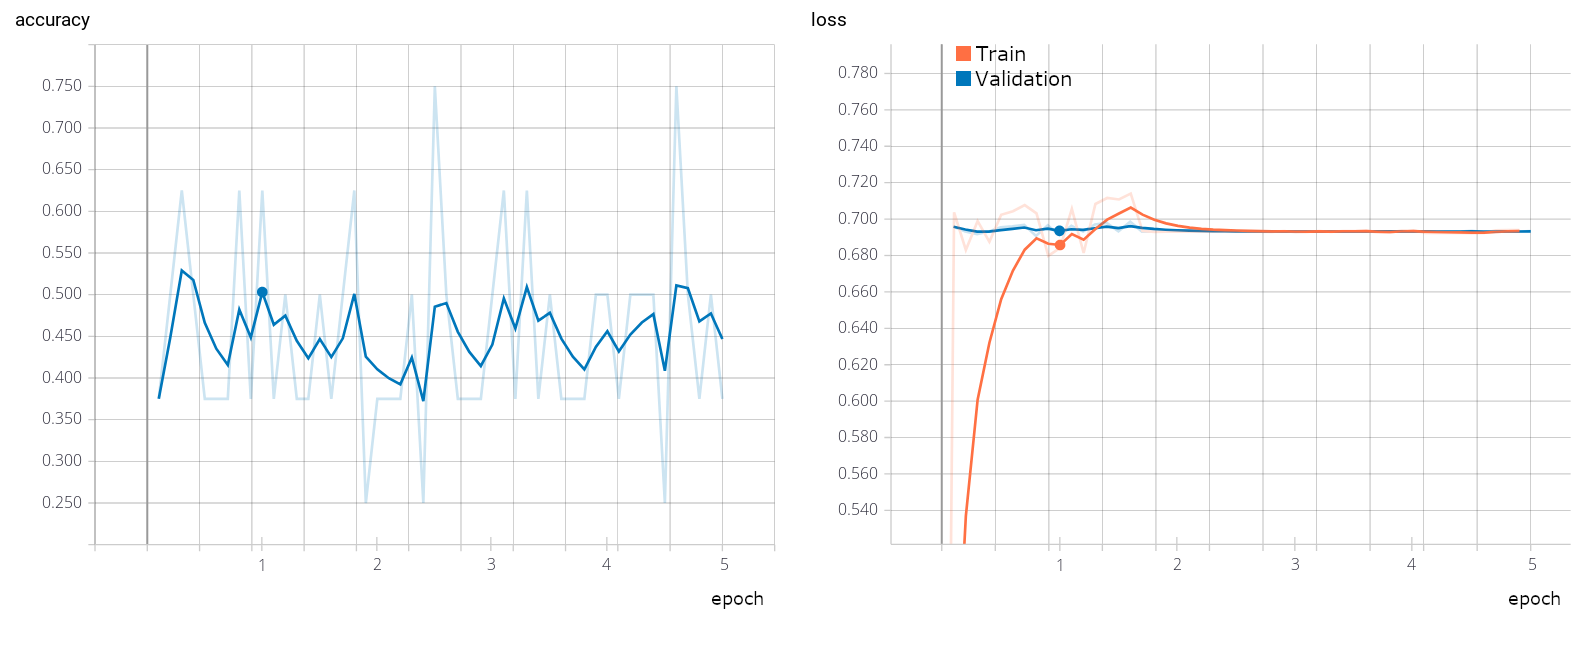
\includegraphics[width=\linewidth]{images/SarrafParkinsonTestResult}
	\caption{Parkinson's disease diagnosis accuracy and loss using Sarraf and Tofighi's algorithm.}
	\label{fig:SarrafParkinsonTestResult}
\end{figure*}


In order to conquer the mentioned downsides of a conventional CNN in Parkinson's disease diagnosis, we will introduce our method which keeps spatial information and can overcome overfitting by reducing model variance. To do so, the proposed algorithm will keep the $z$ index of data and feed them into a 3D Bayesian CNN. As discussed in Section \ref{section:bayesianDL} if we add dropouts before each convolution layer, our model will turn into a deep Bayesian convolutional neural network that can avoid overfitting. Dropouts remove some units (by setting their output values to zero) temporarily which enables other units to justify their weights. Consequently, remaining units in the training phase can precisely adjust their weights to more appropriate ranges if they already hold acceptable values, or keep away from unwanted boundaries noticeably if needed. In addition to that, Bayesian networks are dramatically less compute-intensive and can solve problems in even a single epoch. Hence, a mid-end CPU can be used instead of a high-end GPU in experiments.

As we meant to put temporal data aside, we can assume that the fMRI data for each participant is $t$ different 3D images we had obtained from their brain (despite its time-based sequences). Correspondingly this assumption will multiply our dataset samples by $t (=198)$, enabling us to train our model faster and escape overfitting. On the other hand, in the test phase, our model won't just give binary predictions about a participant being a Parkinson's patient or a healthy control, but it can give us an approximation about the probability of a person being healthy or not. In this step, the trained network will give $t$ different predictions for each person (based on $t$ images) providing a ratio, which corresponds to a probability of healthiness, and we can set a criterion (like $0.5$) to decide if someone belongs to HC class or not.


First of all, input data will be preprocessed using Algorithm \ref{alg:preprocessing}, which removes noises and non-informational data parts (such as the skull). In addition to that, each patient's scan will be normalized to a standard space that boosts the learning phase's efficiency. This step is followed by dividing each sample (containing $t$ 3D fMRI time-slices) to $t$ different images. For instance, in Parkinson's dataset, 30 samples consisted of 198 time-slices of \texttt{$39 \times 64 \times 64$} voxels will turn into $5940$ 3D images. We convert these data to TFRECORD format to improve performance. Furthermore, for each experiment, six participants ($20\%$ of all data) from both groups are randomly selected, and their $t$ time-slices are set aside for the test phase. On the other hand, the rest of the data (which are $24 \times 198$ labeled time-slices) will be shuffled and fed to our 3D deep Bayesian convolutional neural network. We use the first 159 time-slices ($80\%$) as training samples while the remnants will be our validation portion of data correspondingly. 

\begin{algorithm*}
	\caption{Data preparation}
	\label{alg:preprocessing}
	\begin{algorithmic}
		\INPUT{raw fMRI images}
		\STATE 
		\STATE For each fMRI scan following pre-processing steps had been done.
		\STATE 
		
		\item{\textbf{1.}} Intra-modal motion correction using \textbf{MCFLIRT}. it loads the time-series in its entirity and will default to the middle volume as an initial template image. A coarse 8mm search for the motion parameters is then carried out using the cost function specified followed by two subsequent searches at 4mm using increasingly tighter tolerances. All optimizations use trilinear interpolation.
		\STATE 
		
		\item{\textbf{2.}} \textbf{Skull stripping} using BET. Brain Extraction Tool deletes non-brain tissue from an image of the whole head. It can also estimate the inner and outer skull surfaces, and outer scalp surface, if you have good quality T1 and T2 input images.
		\STATE 
		
		\item{\textbf{3.}} \textbf{Spatial Smoothing} via Full-Width at half maximum (FWHM) with 5mm range which is carried out on each volume of the FMRI data set separately. This is intended to reduce noise without reducing valid activation; this is successful as long as the underlying activation area is larger than the extent of the smoothing.
		\STATE 
		
		\item{\textbf{4.}} \textbf{Highpass temporal filtering} uses a local fit of a straight line (Gaussian-weighted within the line to give a smooth response) to remove low frequency artifacts. Low level noises were removed using this filter with $t = 90 sec$.
		\STATE 
		
		\item{\textbf{5.}} The functional images were then aligned to the individual's high-resolution T1-weighted scans, which were subsequently registered to the \textbf{Montreal Neurological Institute standard space (MNI152)} using affine linear registration and resampled at 2mm cubic voxels
		\STATE 

	\end{algorithmic}
\end{algorithm*}


Now we can start to train our model based on the proposed architecture which is illustrated in Figure \ref{fig:cnnArch}. During the training phase, data gets split to 50 chunks ($95$ samples) which are fed sequentially to the network. Consequently, the model can be validated during the training to prevent overfitting and enables us to track the whole process. The proposed method can be briefly expressed as Algorithm \ref{alg:proposedMethod} which $N_{i,p}$ indicates the number of predictions that instance $i$ is a Parkinson's patient and $N_{i,hc}$ indicates a Healthy Control. $\hat{Y}_{i,t}$ is the network prediction for $t$'th time-slice of sample $i$ whilst $Y_i$ is the real class and $C_{i,t}$ is the correctness of that output. Finally, $P_i$ is the predicted probability of how healthy a patient is, $\hat{Y}_i$ is the class based on $P_i$ and $C_i$ is the correctness of that prediction.



\begin{algorithm}
	\caption{Proposed method}
	\label{alg:proposedMethod}
	
	\begin{algorithmic}[1]
		
		\INPUT{processed data which is the output of Algorithm \ref{alg:preprocessing}.}
		\STATE Shuffle scans
		\STATE Put 6 scans (3 group each) aside as test data
		\STATE Split time-slices of data and shuffle them
		\STATE Divide train and validation data to 50 chunks
		\FORALL{50 chunks}  Train network (Fig. \ref{fig:cnnArch}) 
		\STATE Input dropout ($p=0.05$)
		\STATE 3D convolution ($4@64\times64\times39 \;;\; kernel[5,5,5]$)
		\STATE Dropout ($p=0.10$)
		\STATE Max pooling ($4@16\times16\times9 \;;\; pool[4,4,4]$)
		\STATE 3D convolution ($8@16\times16\times9 \;;\; kernel[4,4,4]$)
		\STATE Dropout ($p=0.15$)
		\STATE Max pooling ($8@4\times4\times2 \;;\; pool[4,4,4]$)
		\STATE Dropout ($p=0.20$)
		\STATE Fully connected layer ($16 \; units$)
		\STATE Dropout ($p=0.20$)
		\STATE Fully connected layer ($2 \; units$)
		\STATE Validate and emit network loss and accuracy
		\ENDFOR
		
		\FORALL{test data}
		\STATE $N_{i,p} \gets 0 \;,\; N_{i,hc} \gets 0 \;,\; C_{i,t} \gets 0$
		\FORALL{time-slices}
		\IF {$\hat{Y}_{i,t} =\; $Parkinson's} 
		\STATE $N_{i,p} \gets N_{i,p} + 1$
		\ELSE
		\STATE $N_{i,hc} \gets N_{i,hc} + 1$
		\ENDIF
		
		\IF {$\hat{Y}_{i,t} = Y_i$} 
		\STATE $C_{i,t} \gets 1$
		\ELSE 
		\STATE $C_{i,t} \gets 0$
		\ENDIF
		\ENDFOR
		
		\STATE ${P_{i}} \gets {N_{i,hc} \over T_{(=198)}}$
		
		\IF {$ P_{i} \geq 0.5$}
		\STATE $\hat{Y}_i \gets \;$ Healthy Control
		\ELSE
		\STATE $\hat{Y}_i \gets \;$ Parkinson's
		\ENDIF
		
		\IF {$\hat{Y}_{i} = Y_{i}$} 
		\STATE $C_{i} \gets 1$
		\ELSE
		\STATE $C_{i} \gets 0$
		\ENDIF
		
		\ENDFOR
		
		%\IF {$i\geq 5$} 
		%\STATE $i\gets i-1$
		%\ELSE
		%\IF {$i\leq 3$}
		%\STATE $i\gets i+2$
		%\ENDIF
		%\ENDIF 
	\end{algorithmic}
	
	%	\KwData{pre-processed data which is the output of Algorithm \ref{alg:preprocessing}.}
	%	\KwResult{trained Bayesian 3D CNN to diagnose Parkinson's disease patients}
	%	initialization\;
	%	\While{not at end of this document}{
	%		read current\;
	%		\eIf{understand}{
	%			go to next section\;
	%			current section becomes this one\;
	%		}{
	%			go back to the beginning of current section\;
	%		}
	%	}
	
\end{algorithm}



Furthermore, our model's accuracy can be obtained in two different aspects. The first one would be the correctness of each time-slice prediction ($\overline{C}_{T}$), while the second, is the accuracy of disease diagnosis ($\overline{C}$), and we are mostly interested in the later. Both of the mentioned statistics can be calculated using Equations \eqref{eq:meanTimeSliceCorrectness} and \eqref{eq:meanCorrectness}.


\begin{figure*}
	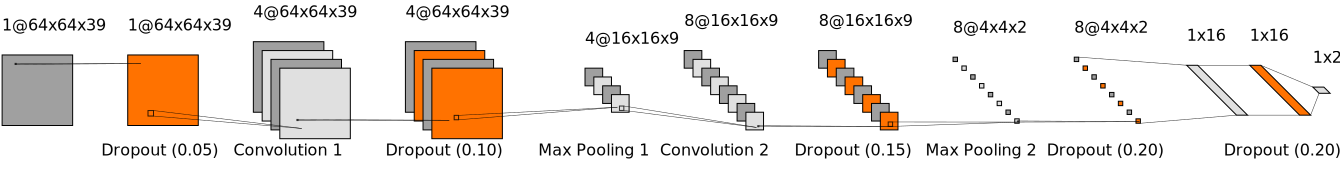
\includegraphics[width=\linewidth]{images/cnnArchHorizontal}
	\caption{Proposed architecture}
	\label{fig:cnnHorizontalArch}
\end{figure*}

\begin{eqnarray}
\label{eq:meanTimeSliceCorrectness}
\overline{C_{T}} &=& {{\sum_{i=1}^{m} \sum_{t=1}^{T (=198)} C_{i,t} } \over {m \times T} } \\ 
\label{eq:meanCorrectness}
\overline{C} &=& {{\sum_{i=1}^{m} C_i } \over {m } } 
\end{eqnarray}



As can be seen in Figure \ref{fig:cnnHorizontalArch}, we have added different dropout units between our convolution and pooling layers to avoid overfitting, decrease variance and make convergence to appropriate weights faster. In addition to that, dropout probabilities increase in each layer because layers with less free parameters have a greater chance to train well even if they are less frequently updated. In other words, a huge number of parameters cannot tune acceptably with a small amount of data while getting omitted a lot. On the other hand, as there are only 16 weights in the first fully connected layer, higher dropout probabilities can speed up the training process.






\section{Experiments and results}
\label{section:results}
As discussed in Section \ref{section:proposedMethod}, our method does not demand high processing power so we can use a CPU for our experiments. All of the tests had been run on an Intel\textsuperscript{\tiny\textregistered} 4710HQ CPU. Averagely, the training phase takes $1h \; 12m \; 4s$ and the test phase finishes in $6m \; 41s$. Also it worth mentioning that the application consumes 270 megabytes of RAM thanks to the TFRECORD file format.

Table \ref{table:averageAccuracies} shows a summary of 8 different tests. We can define the average of mean accuracies as Equations \eqref{eq:averageMeanTimeSliceCorrectness} and \eqref{eq:averageMeanCorrectness} in order to use them as a measure that shows how the model is performing in the case of accuracy. 

\begin{eqnarray}
\label{eq:averageMeanTimeSliceCorrectness}
\mathbf{C_t} &=& {{\sum_{j=1}^{J} \overline{C_{T}} } \over {J} } \\ 
\label{eq:averageMeanCorrectness}
\mathbf{C} &=& {{\sum_{j=1}^{J} \overline{C} } \over {J} } 
\end{eqnarray}


\begin{table}
	\caption{Average accuracies for different tests}
	\begin{tabular}{| c | c | c| }
		\hline
		$j$ & $\overline{C_{i,t}}\;(\%)$ & $\overline{C_i}\;(\%)$ \\ 
		test no. & mean time-slice accuracy & mean accuracy \\ \hline
		1 & 100 & 100 \\
		2 & 97.90 & 100 \\
		3 & 74.83 & 83.33 \\
		4 & 96.30 & 100 \\
		5 & 97.14 & 100 \\
		6 & 100 & 100 \\
		7 & 98.65 & 100 \\
		8 & 85.35 & 100 \\ \hline
		Average & $\mathbf{C_t} = $ 93.77 & $\mathbf{C} = $ 97.92 \\
		\hline
	\end{tabular}
\label{table:averageAccuracies}
\end{table}

As we can see, the proposed method has shown huge success in the task of Parkinson's disease diagnosis in an affordable time. Also, the fascinating point about the experiments is the average mean time-slice accuracy, which is around $92.96\%$. Accordingly, it means the model is able to judge only by a single time-slice of the brain while the prediction is acceptably accurate. We mostly care about the average mean accuracy, which is the average accuracy of the disease diagnosis task and as long as the whole process can predict someone's health situation precisely, we can ignore the time-slice based results. So, we should mostly focus on average mean accuracy and use that to compare the proposed method to other models. 




\begin{table}
	\caption{Test results for experiment 1. HC stands for Health Control while P means Parkinson's disease}
	\resizebox{\linewidth}{!}{%
		\begin{tabular}{ | c | c | c | c | c | c | c | c | }
			\hline
			patient & $Y_i$ & $N_{hc}$ & $N_p$ & $C_{i,t} (\%)$ & $P_i$ & $\hat{Y}_i$ & $C_i (\%)$ \\  \hline
			CTL04 & HC & 198 &  0  & 100 & 1 & HC & 100 \\
			CTL05 & HC & 198 &  0  & 100 & 1 & HC & 100 \\
			CTL02 & HC & 198 &  0  & 100 & 1 & HC & 100 \\
			ODP04 & P   &  0  & 198 & 100 & 0 &  P  & 100 \\
			ODP05 & P   &  0  & 198 & 100 & 0 &  P  & 100 \\
			ODP02 & P   &  0  & 198 & 100 & 0 &  P  & 100 \\ \hline
			\multicolumn{4}{|r|}{\tiny{Mean time-slice accuracy} $\overline{C_{i,t}}$} & 100 &
			\multicolumn{2}{|r|}{\tiny{Mean accuracy} $\overline{C_{i}}$} & 100 \\
			\hline \hline
			
			\multicolumn{2}{|r|}{True positive (TP)} & 
			\multicolumn{2}{c|}{ 3 } &
			\multicolumn{2}{|r|}{False positive (FP)} & 
			\multicolumn{2}{c|}{ 0 } \\ 
			\multicolumn{2}{|r|}{False negative (FN)} & 
			\multicolumn{2}{c|}{ 0 } &
			\multicolumn{2}{|r|}{True negative (TN)} & 
			\multicolumn{2}{c|}{ 3 }  \\
			\hline \hline
			
			\multicolumn{2}{|r|}{Time-slice TP} & 
			\multicolumn{2}{c|}{ 594 } &
			\multicolumn{2}{|r|}{Time-slice FP} & 
			\multicolumn{2}{c|}{ 0 } \\ 
			\multicolumn{2}{|r|}{Time-slice FN} & 
			\multicolumn{2}{c|}{ 0 } &
			\multicolumn{2}{|r|}{Time-slice TN} & 
			\multicolumn{2}{c|}{ 594 }  \\
			\hline \hline
			
			\multicolumn{2}{|r|}{Time-slice sensitivity} & 
			\multicolumn{2}{c|}{ 1 } &
			\multicolumn{2}{|r|}{Sensitivity} & 
			\multicolumn{2}{c|}{ 1 } \\ 
			
			\multicolumn{2}{|r|}{Time-slice specificity} & 
			\multicolumn{2}{c|}{ 1 } &
			\multicolumn{2}{|r|}{Specificity} & 
			\multicolumn{2}{c|}{ 1 } \\ 
			
			\multicolumn{2}{|r|}{Time-slice PPV} & 
			\multicolumn{2}{c|}{ 1 } &
			\multicolumn{2}{|r|}{PPV} & 
			\multicolumn{2}{c|}{ 1 } \\ 
			
			\multicolumn{2}{|r|}{Time-slice NPV} & 
			\multicolumn{2}{c|}{ 1 } &
			\multicolumn{2}{|r|}{NPV} & 
			\multicolumn{2}{c|}{ 1 } \\ \hline
		\end{tabular}
	}
	\label{table:tests_1}
\end{table}
\begin{figure}
	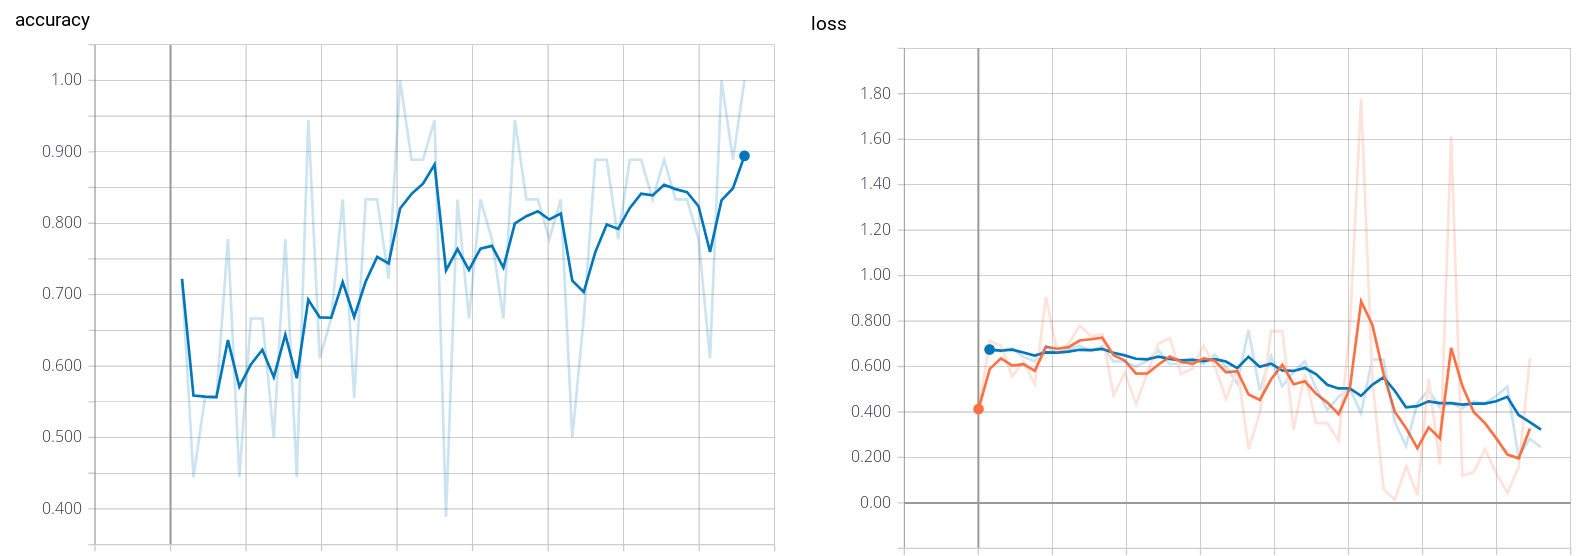
\includegraphics[width=\linewidth]{images/tests_1}
	\caption{Experiment 1. Accuracy and loss of network for training and validation data. Accuracy is based on validation data and loss diagram contains train data loss in blue and validation loss in orange.}
	\label{fig:tests_1}
\end{figure}




\begin{table}
	\caption{Test results for experiment 2.}
	\resizebox{\linewidth}{!}{%
		\begin{tabular}{ | c | c | c | c | c | c | c | c | }
			\hline
			patient & $Y_i$ & $N_{hc}$ & $N_p$ & $C_{i,t} (\%)$ & $P_i$ & $\hat{Y}_i$ & $C_i (\%)$ \\  \hline
			CTL08 & HC & 191 &  7  & 96.46 & 0.9646 & HC & 100 \\
			CTL12 & HC & 195 &  3  & 98.48 & 0.9848 & HC & 100 \\
			CTL01 & HC & 198 &  0  & 100 & 1 & HC & 100 \\
			ODP08 & P   &  1  & 197 & 99.49 & 0.0050 &  P  & 100 \\
			ODP12 & P   &  2  & 196 & 98.99 & 0.0101 &  P  & 100 \\
			ODP01 & P   &  12  & 186 & 93.94 & 0.0606 &  P  & 100 \\ \hline
			\multicolumn{4}{|r|}{$\overline{C_{i,t}}$} & 97.90 &
			\multicolumn{2}{|r|}{$\overline{C_{i}}$} & 100 \\
			\hline \hline
			
			\multicolumn{2}{|r|}{True positive (TP)} & 
			\multicolumn{2}{c|}{ 3 } &
			\multicolumn{2}{|r|}{False positive (FP)} & 
			\multicolumn{2}{c|}{ 0 } \\ 
			\multicolumn{2}{|r|}{False negative (FN)} & 
			\multicolumn{2}{c|}{ 0 } &
			\multicolumn{2}{|r|}{True negative (TN)} & 
			\multicolumn{2}{c|}{ 3 }  \\
			\hline \hline
			
			\multicolumn{2}{|r|}{Time-slice TP} & 
			\multicolumn{2}{c|}{ 584 } &
			\multicolumn{2}{|r|}{Time-slice FP} & 
			\multicolumn{2}{c|}{ 15 } \\ 
			\multicolumn{2}{|r|}{Time-slice FN} & 
			\multicolumn{2}{c|}{ 10 } &
			\multicolumn{2}{|r|}{Time-slice TN} & 
			\multicolumn{2}{c|}{ 579 }  \\
			\hline \hline
			
			\multicolumn{2}{|r|}{Time-slice sensitivity} & 
			\multicolumn{2}{c|}{ 0.983164983 } &
			\multicolumn{2}{|r|}{Sensitivity} & 
			\multicolumn{2}{c|}{ 1 } \\ 
			
			\multicolumn{2}{|r|}{Time-slice specificity} & 
			\multicolumn{2}{c|}{ 0.974747475 } &
			\multicolumn{2}{|r|}{Specificity} & 
			\multicolumn{2}{c|}{ 1 } \\ 
			
			\multicolumn{2}{|r|}{Time-slice PPV} & 
			\multicolumn{2}{c|}{ 0.974958264 } &
			\multicolumn{2}{|r|}{PPV} & 
			\multicolumn{2}{c|}{ 1 } \\ 
			
			\multicolumn{2}{|r|}{Time-slice NPV} & 
			\multicolumn{2}{c|}{ 0.983022071 } &
			\multicolumn{2}{|r|}{NPV} & 
			\multicolumn{2}{c|}{ 1 } \\ \hline
		\end{tabular}
	}
	\label{table:tests_2}
\end{table}
\begin{figure}
	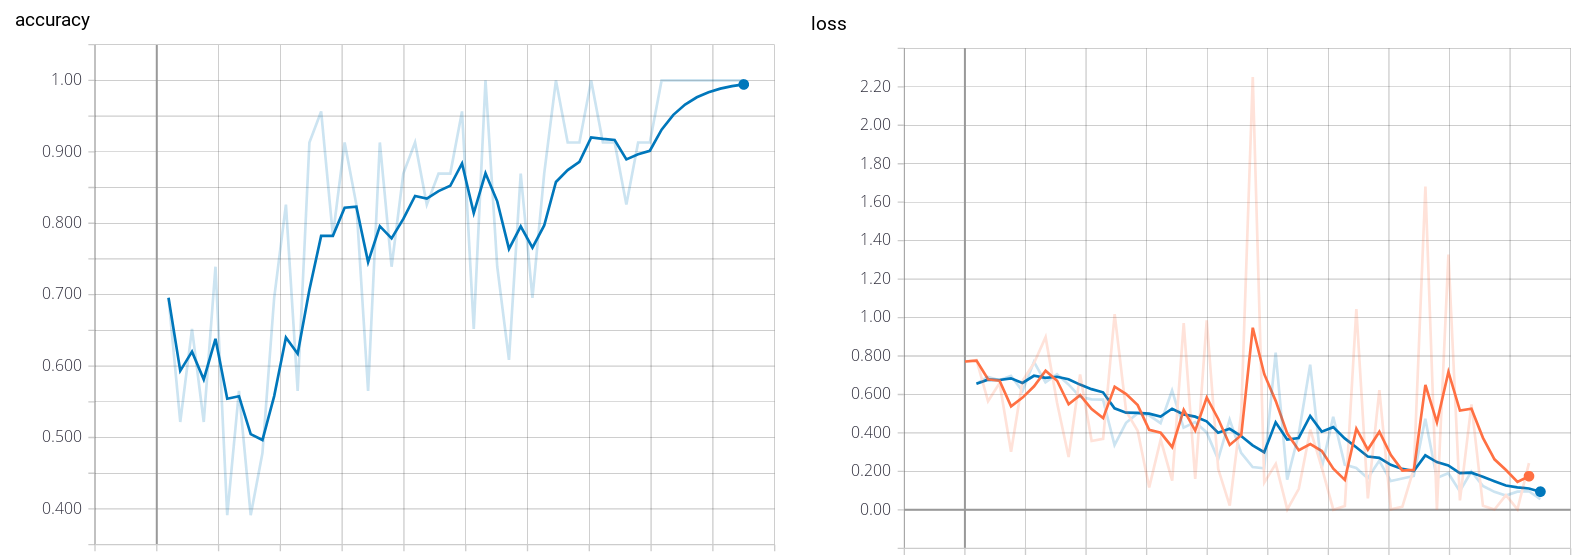
\includegraphics[width=\linewidth]{images/tests_2}
	\caption{Experiment 2. Accuracy and loss of network for training and validation data.}
	\label{fig:tests_2}
\end{figure}




\begin{table}
\caption{Test results for experiment 3.}
\resizebox{\linewidth}{!}{%
	\begin{tabular}{ | c | c | c | c | c | c | c | c | }
		\hline
		patient & $Y_i$ & $N_{hc}$ & $N_p$ & $C_{i,t} (\%)$ & $P_i$ & $\hat{Y}_i$ & $C_i (\%)$ \\  \hline
		CTL03 & HC & 198 &  0   &   100   &     1      & HC & 100 \\
		CTL13 & HC & 198 &  0   &   100   &     1      & HC & 100 \\
		CTL14 & HC & 198 &  0   &   100   &     1      & HC & 100 \\
		ODP03 & P  &  53  & 145 & 73.23 & 0.2677 &  P  & 100 \\
		ODP13 & P  & 198 &   0   &     0    &      1      & HC  & 0 \\
		ODP14 & P  & 48  &  150 & 75.76  & 0.2424 &  P  & 100 \\ \hline
		\multicolumn{4}{|r|}{$\overline{C_{i,t}}$} & 74.83 &
		\multicolumn{2}{|r|}{$\overline{C_{i}}$} & 83.33 \\
		\hline \hline
		
		\multicolumn{2}{|r|}{True positive (TP)} & 
		\multicolumn{2}{c|}{ 3 } &
		\multicolumn{2}{|r|}{False positive (FP)} & 
		\multicolumn{2}{c|}{ 1 } \\ 
		\multicolumn{2}{|r|}{False negative (FN)} & 
		\multicolumn{2}{c|}{ 0 } &
		\multicolumn{2}{|r|}{True negative (TN)} & 
		\multicolumn{2}{c|}{ 2 }  \\
		\hline \hline
		
		\multicolumn{2}{|r|}{Time-slice TP} & 
		\multicolumn{2}{c|}{ 594 } &
		\multicolumn{2}{|r|}{Time-slice FP} & 
		\multicolumn{2}{c|}{ 299 } \\ 
		\multicolumn{2}{|r|}{Time-slice FN} & 
		\multicolumn{2}{c|}{ 0 } &
		\multicolumn{2}{|r|}{Time-slice TN} & 
		\multicolumn{2}{c|}{ 295 }  \\
		\hline \hline
		
		\multicolumn{2}{|r|}{Time-slice sensitivity} & 
		\multicolumn{2}{c|}{ 1 } &
		\multicolumn{2}{|r|}{Sensitivity} & 
		\multicolumn{2}{c|}{ 1 } \\ 
		
		\multicolumn{2}{|r|}{Time-slice specificity} & 
		\multicolumn{2}{c|}{ 0.496632997 } &
		\multicolumn{2}{|r|}{Specificity} & 
		\multicolumn{2}{c|}{ 0.666666667 } \\ 
		
		\multicolumn{2}{|r|}{Time-slice PPV} & 
		\multicolumn{2}{c|}{ 0.665173572 } &
		\multicolumn{2}{|r|}{PPV} & 
		\multicolumn{2}{c|}{ 0.75 } \\ 
		
		\multicolumn{2}{|r|}{Time-slice NPV} & 
		\multicolumn{2}{c|}{ 1 } &
		\multicolumn{2}{|r|}{NPV} & 
		\multicolumn{2}{c|}{ 1 } \\ \hline
	\end{tabular}
}
\label{table:tests_3}
\end{table}
\begin{figure}
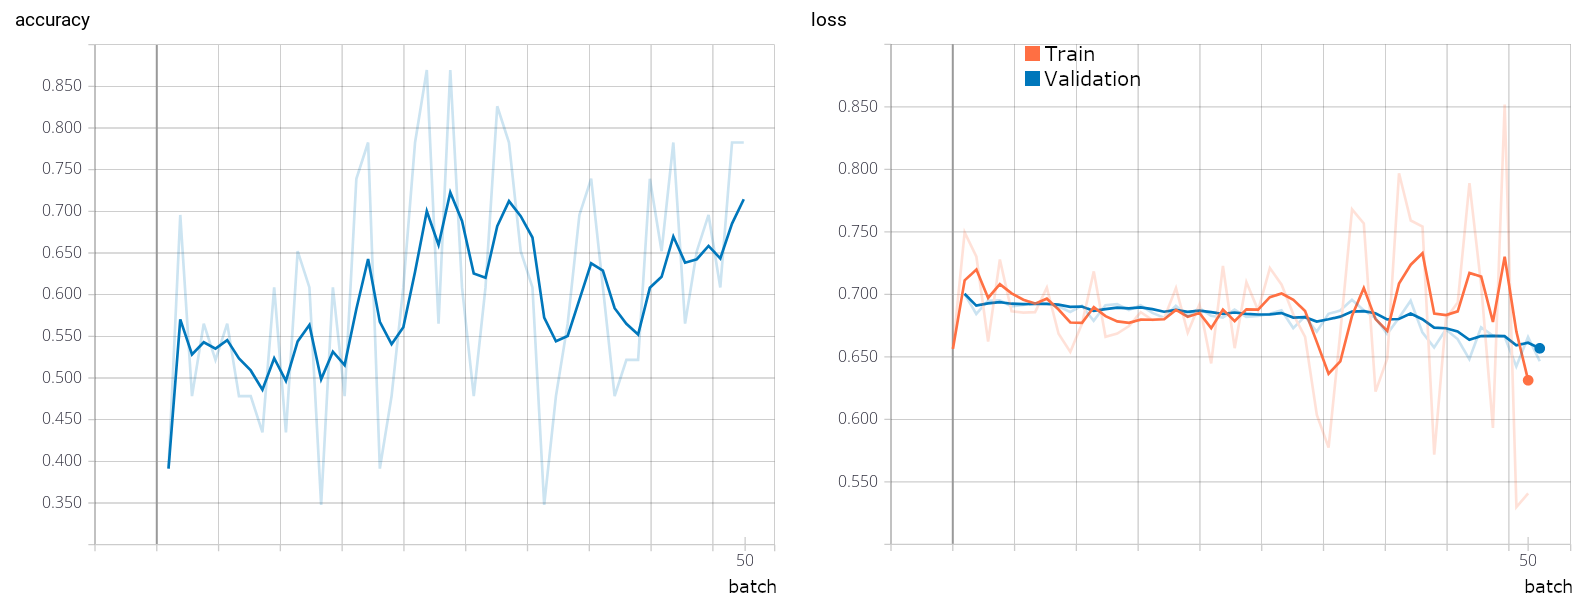
\includegraphics[width=\linewidth]{images/tests_3}
\caption{Experiment 3. Accuracy and loss of network for training and validation data.}
\label{fig:tests_3}
\end{figure}




\begin{table}
\caption{Test results for experiment 4.}
\resizebox{\linewidth}{!}{%
	\begin{tabular}{ | c | c | c | c | c | c | c | c | }
		\hline
		patient & $Y_i$ & $N_{hc}$ & $N_p$ & $C_{i,t} (\%)$ & $P_i$ & $\hat{Y}_i$ & $C_i (\%)$ \\  \hline
		CTL12 & HC & 185 & 13  & 93.43 & 0.9343 & HC & 100 \\
		CTL06 & HC & 197 &  1   & 99.49 & 0.9949 & HC & 100 \\
		CTL11 & HC & 170 & 28  & 85.86 & 0.8586 & HC & 100 \\
		ODP12 & P  &   0   & 198 &  100   &      0     &  P  & 100 \\
		ODP06 & P  &   0   & 198 &  100   &      0     &  P  & 100 \\
		ODP11 & P  &   2   & 196 & 98.99 & 0.0101  &  P  & 100 \\ \hline
		\multicolumn{4}{|r|}{$\overline{C_{i,t}}$} & 96.30 &
		\multicolumn{2}{|r|}{$\overline{C_{i}}$} & 100  \\
		\hline \hline
		
		\multicolumn{2}{|r|}{True positive (TP)} & 
		\multicolumn{2}{c|}{ 3 } &
		\multicolumn{2}{|r|}{False positive (FP)} & 
		\multicolumn{2}{c|}{ 0 } \\ 
		\multicolumn{2}{|r|}{False negative (FN)} & 
		\multicolumn{2}{c|}{ 0 } &
		\multicolumn{2}{|r|}{True negative (TN)} & 
		\multicolumn{2}{c|}{ 3 }  \\
		\hline \hline
		
		\multicolumn{2}{|r|}{Time-slice TP} & 
		\multicolumn{2}{c|}{ 552 } &
		\multicolumn{2}{|r|}{Time-slice FP} & 
		\multicolumn{2}{c|}{ 2 } \\ 
		\multicolumn{2}{|r|}{Time-slice FN} & 
		\multicolumn{2}{c|}{ 42 } &
		\multicolumn{2}{|r|}{Time-slice TN} & 
		\multicolumn{2}{c|}{ 592 }  \\
		\hline \hline
		
		\multicolumn{2}{|r|}{Time-slice sensitivity} & 
		\multicolumn{2}{c|}{ 0.929292929 } &
		\multicolumn{2}{|r|}{Sensitivity} & 
		\multicolumn{2}{c|}{ 1 } \\ 
		
		\multicolumn{2}{|r|}{Time-slice specificity} & 
		\multicolumn{2}{c|}{ 0.996632997 } &
		\multicolumn{2}{|r|}{Specificity} & 
		\multicolumn{2}{c|}{ 1 } \\ 
		
		\multicolumn{2}{|r|}{Time-slice PPV} & 
		\multicolumn{2}{c|}{ 0.996389892 } &
		\multicolumn{2}{|r|}{PPV} & 
		\multicolumn{2}{c|}{ 1 } \\ 
		
		\multicolumn{2}{|r|}{Time-slice NPV} & 
		\multicolumn{2}{c|}{ 0.933753943 } &
		\multicolumn{2}{|r|}{NPV} & 
		\multicolumn{2}{c|}{ 1 } \\ \hline
	\end{tabular}
}
\label{table:tests_4}
\end{table}
\begin{figure}
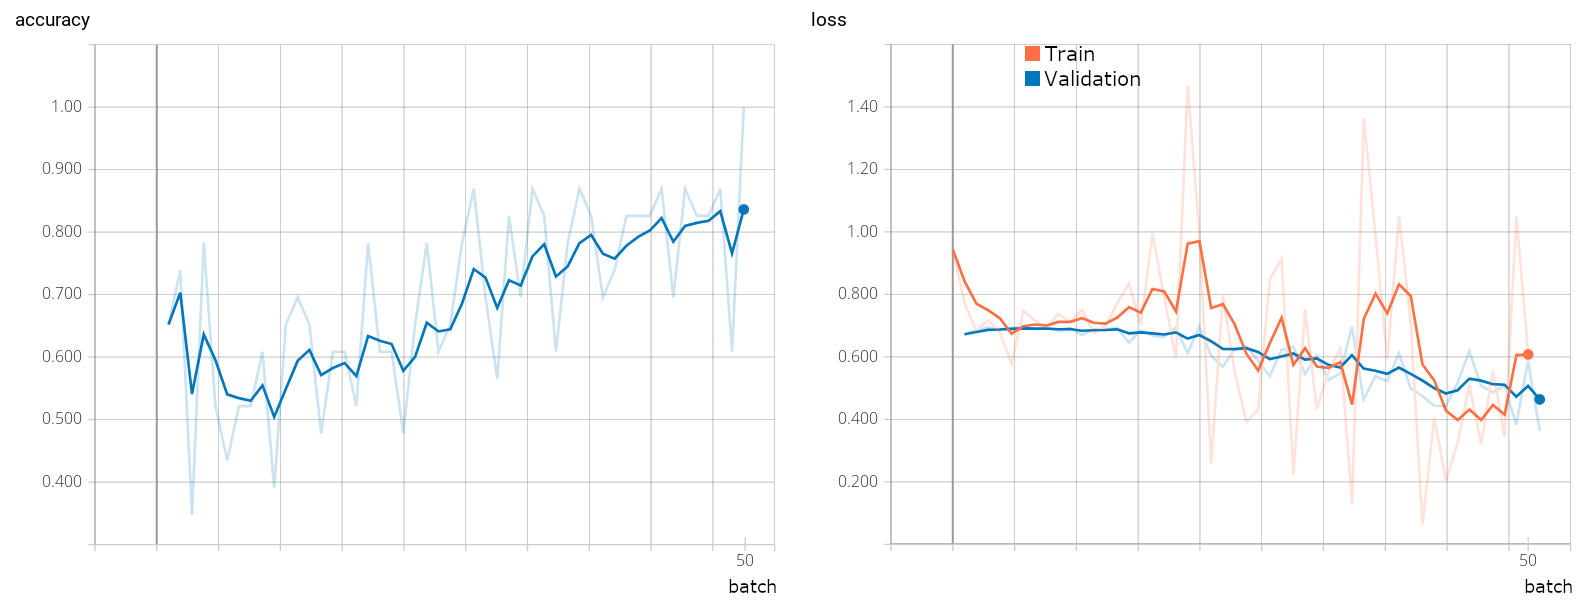
\includegraphics[width=\linewidth]{images/tests_4}
\caption{Experiment 4. Accuracy and loss of network for training and validation data.}
\label{fig:tests_4}
\end{figure}




\begin{table}
\caption{Test results for experiment 5.}
\resizebox{\linewidth}{!}{%
	\begin{tabular}{ | c | c | c | c | c | c | c | c | }
		\hline
		patient & $Y_i$ & $N_{hc}$ & $N_p$ & $C_{i,t} (\%)$ & $P_i$ & $\hat{Y}_i$ & $C_i (\%)$ \\  \hline
		CTL15 & HC & 198 &   0   &  100  & 1 & HC & 100 \\
		CTL11 & HC & 198  &   0   &  100  & 1 & HC & 100 \\
		CTL07 & HC & 198 &   0   &  100  & 1 & HC & 100 \\
		ODP15 & P   &   0   & 198 &  100  & 0 &  P  & 100 \\
		ODP11 & P   &  34  &  164 &82.83& 0.1717 &  P  & 100 \\
		ODP07 & P  &   0   &  198 & 1 00  &0  &  P  & 100 \\ \hline
		\multicolumn{4}{|r|}{$\overline{C_{i,t}}$} & 97.14 &
		\multicolumn{2}{|r|}{$\overline{C_{i}}$} & 100 \\
		\hline \hline
		
		\multicolumn{2}{|r|}{True positive (TP)} & 
		\multicolumn{2}{c|}{ 3 } &
		\multicolumn{2}{|r|}{False positive (FP)} & 
		\multicolumn{2}{c|}{ 0 } \\ 
		\multicolumn{2}{|r|}{False negative (FN)} & 
		\multicolumn{2}{c|}{ 0 } &
		\multicolumn{2}{|r|}{True negative (TN)} & 
		\multicolumn{2}{c|}{ 3 }  \\
		\hline \hline
		
		\multicolumn{2}{|r|}{Time-slice TP} & 
		\multicolumn{2}{c|}{ 594 } &
		\multicolumn{2}{|r|}{Time-slice FP} & 
		\multicolumn{2}{c|}{ 34 } \\ 
		\multicolumn{2}{|r|}{Time-slice FN} & 
		\multicolumn{2}{c|}{ 0 } &
		\multicolumn{2}{|r|}{Time-slice TN} & 
		\multicolumn{2}{c|}{ 560 }  \\
		\hline \hline
		
		\multicolumn{2}{|r|}{Time-slice sensitivity} & 
		\multicolumn{2}{c|}{ 1 } &
		\multicolumn{2}{|r|}{Sensitivity} & 
		\multicolumn{2}{c|}{ 1 } \\ 
		
		\multicolumn{2}{|r|}{Time-slice specificity} & 
		\multicolumn{2}{c|}{ 0.942760943 } &
		\multicolumn{2}{|r|}{Specificity} & 
		\multicolumn{2}{c|}{ 1 } \\ 
		
		\multicolumn{2}{|r|}{Time-slice PPV} & 
		\multicolumn{2}{c|}{ 0.945859873 } &
		\multicolumn{2}{|r|}{PPV} & 
		\multicolumn{2}{c|}{ 1 } \\ 
		
		\multicolumn{2}{|r|}{Time-slice NPV} & 
		\multicolumn{2}{c|}{ 1 } &
		\multicolumn{2}{|r|}{NPV} & 
		\multicolumn{2}{c|}{ 1 } \\ \hline
	\end{tabular}
}
\label{table:tests_5}
\end{table}
\begin{figure}
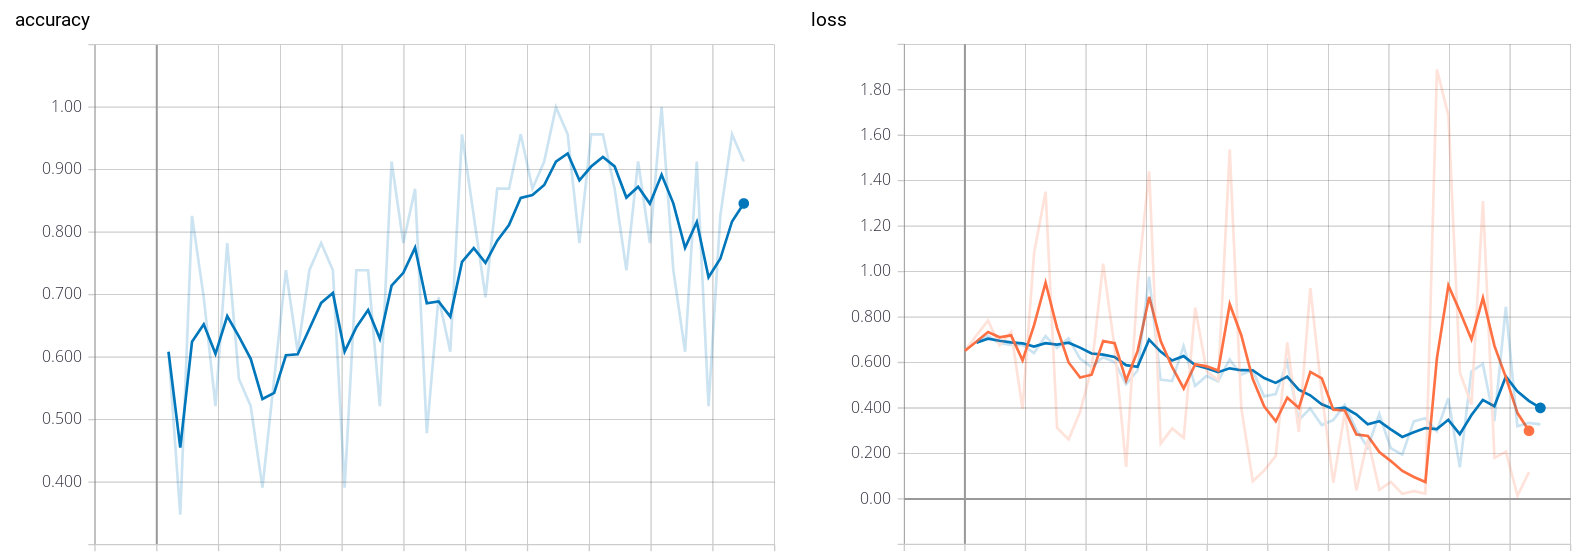
\includegraphics[width=\linewidth]{images/tests_5}
\caption{Experiment 5. Accuracy and loss of network for training and validation data.}
\label{fig:tests_5}
\end{figure}




\begin{table}
\caption{Test results for experiment 6.}
\resizebox{\linewidth}{!}{%
	\begin{tabular}{ | c | c | c | c | c | c | c | c | }
		\hline
		patient & $Y_i$ & $N_{hc}$ & $N_p$ & $C_{i,t} (\%)$ & $P_i$ & $\hat{Y}_i$ & $C_i (\%)$ \\  \hline
		CTL10 & HC & 198 &  0 & 100 & 1 & HC & 100 \\
		CTL03 & HC & 198 &  0 & 100 & 1 & HC & 100 \\
		CTL02 & HC & 198 &  0 & 100 & 1 & HC & 100 \\
		ODP10 & P  &  0  & 198 & 100 & 0 &  P  & 100 \\
		ODP03 & P  &  0  & 198 & 100 & 0 &  P  & 100 \\
		ODP02 & P  &  0  & 198 & 100 & 0 &  P  & 100 \\ \hline
		\multicolumn{4}{|r|}{$\overline{C_{i,t}}$} & 100 &
		\multicolumn{2}{|r|}{$\overline{C_{i}}$} & 100 \\
		\hline \hline
		
		\multicolumn{2}{|r|}{True positive (TP)} & 
		\multicolumn{2}{c|}{ 3 } &
		\multicolumn{2}{|r|}{False positive (FP)} & 
		\multicolumn{2}{c|}{ 0 } \\ 
		\multicolumn{2}{|r|}{False negative (FN)} & 
		\multicolumn{2}{c|}{ 0 } &
		\multicolumn{2}{|r|}{True negative (TN)} & 
		\multicolumn{2}{c|}{ 3 }  \\
		\hline \hline
		
		\multicolumn{2}{|r|}{Time-slice TP} & 
		\multicolumn{2}{c|}{ 594 } &
		\multicolumn{2}{|r|}{Time-slice FP} & 
		\multicolumn{2}{c|}{ 0 } \\ 
		\multicolumn{2}{|r|}{Time-slice FN} & 
		\multicolumn{2}{c|}{ 0 } &
		\multicolumn{2}{|r|}{Time-slice TN} & 
		\multicolumn{2}{c|}{ 594 }  \\
		\hline \hline
		
		\multicolumn{2}{|r|}{Time-slice sensitivity} & 
		\multicolumn{2}{c|}{ 1 } &
		\multicolumn{2}{|r|}{Sensitivity} & 
		\multicolumn{2}{c|}{ 1 } \\ 
		
		\multicolumn{2}{|r|}{Time-slice specificity} & 
		\multicolumn{2}{c|}{ 1 } &
		\multicolumn{2}{|r|}{Specificity} & 
		\multicolumn{2}{c|}{ 1 } \\ 
		
		\multicolumn{2}{|r|}{Time-slice PPV} & 
		\multicolumn{2}{c|}{ 1 } &
		\multicolumn{2}{|r|}{PPV} & 
		\multicolumn{2}{c|}{ 1 } \\ 
		
		\multicolumn{2}{|r|}{Time-slice NPV} & 
		\multicolumn{2}{c|}{ 1 } &
		\multicolumn{2}{|r|}{NPV} & 
		\multicolumn{2}{c|}{ 1 } \\ \hline
	\end{tabular}
}
\label{table:tests_6}
\end{table}
\begin{figure}
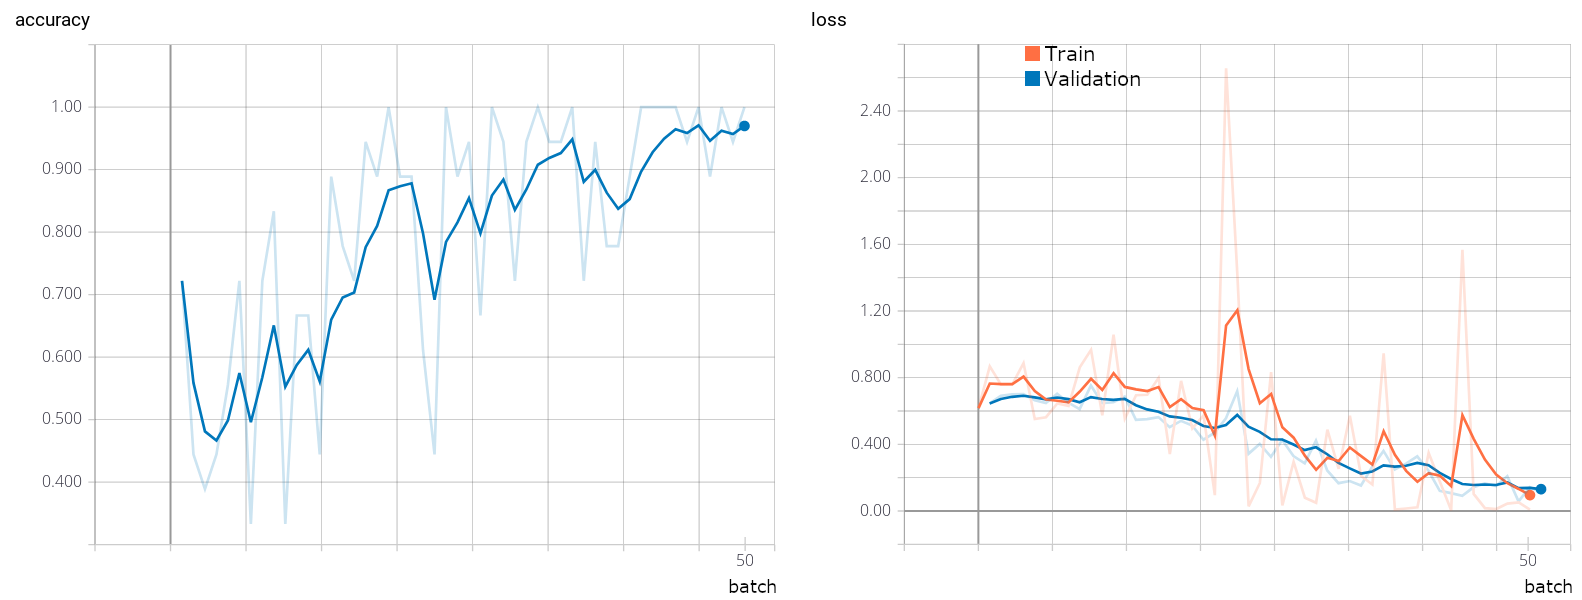
\includegraphics[width=\linewidth]{images/tests_6}
\caption{Experiment 6. Accuracy and loss of network for training and validation data.}
\label{fig:tests_6}
\end{figure}




\begin{table}
\caption{Test results for experiment 7.}
\resizebox{\linewidth}{!}{%
	\begin{tabular}{ | c | c | c | c | c | c | c | c | }
		\hline
		patient & $Y_i$ & $N_{hc}$ & $N_p$ & $C_{i,t} (\%)$ & $P_i$ & $\hat{Y}_i$ & $C_i (\%)$ \\  \hline
		CTL05 & HC & 194 &  4   & 97.98 & 0.9798 & HC & 100 \\
		CTL04 & HC & 198 &  0   &   100  &      1     & HC & 100 \\
		CTL10 & HC & 186  &  12 & 93.94 & 0.9394 & HC & 100 \\
		ODP05 & P  &   0   & 198 &   100  &     0     &  P  & 100 \\
		ODP04 & P  &   0   & 198 &   100  &     0     &  P  & 100 \\
		ODP10 & P  &   0    & 198 &   100  &    0      &  P  & 100 \\ \hline
		\multicolumn{4}{|r|}{$\overline{C_{i,t}}$} & 98.65 &
		\multicolumn{2}{|r|}{$\overline{C_{i}}$} & 100 \\
		\hline \hline
		
		\multicolumn{2}{|r|}{True positive (TP)} & 
		\multicolumn{2}{c|}{ 3 } &
		\multicolumn{2}{|r|}{False positive (FP)} & 
		\multicolumn{2}{c|}{ 0 } \\ 
		\multicolumn{2}{|r|}{False negative (FN)} & 
		\multicolumn{2}{c|}{ 0 } &
		\multicolumn{2}{|r|}{True negative (TN)} & 
		\multicolumn{2}{c|}{ 3 }  \\
		\hline \hline
		
		\multicolumn{2}{|r|}{Time-slice TP} & 
		\multicolumn{2}{c|}{ 578 } &
		\multicolumn{2}{|r|}{Time-slice FP} & 
		\multicolumn{2}{c|}{ 0 } \\ 
		\multicolumn{2}{|r|}{Time-slice FN} & 
		\multicolumn{2}{c|}{ 16 } &
		\multicolumn{2}{|r|}{Time-slice TN} & 
		\multicolumn{2}{c|}{ 594 }  \\
		\hline \hline
		
		\multicolumn{2}{|r|}{Time-slice sensitivity} & 
		\multicolumn{2}{c|}{ 0.973063973 } &
		\multicolumn{2}{|r|}{Sensitivity} & 
		\multicolumn{2}{c|}{ 1 } \\ 
		
		\multicolumn{2}{|r|}{Time-slice specificity} & 
		\multicolumn{2}{c|}{ 1 } &
		\multicolumn{2}{|r|}{Specificity} & 
		\multicolumn{2}{c|}{ 1 } \\ 
		
		\multicolumn{2}{|r|}{Time-slice PPV} & 
		\multicolumn{2}{c|}{ 1 } &
		\multicolumn{2}{|r|}{PPV} & 
		\multicolumn{2}{c|}{ 1 } \\ 
		
		\multicolumn{2}{|r|}{Time-slice NPV} & 
		\multicolumn{2}{c|}{ 0.973770492 } &
		\multicolumn{2}{|r|}{NPV} & 
		\multicolumn{2}{c|}{ 1 } \\ \hline
	\end{tabular}
}
\label{table:tests_7}
\end{table}
\begin{figure}
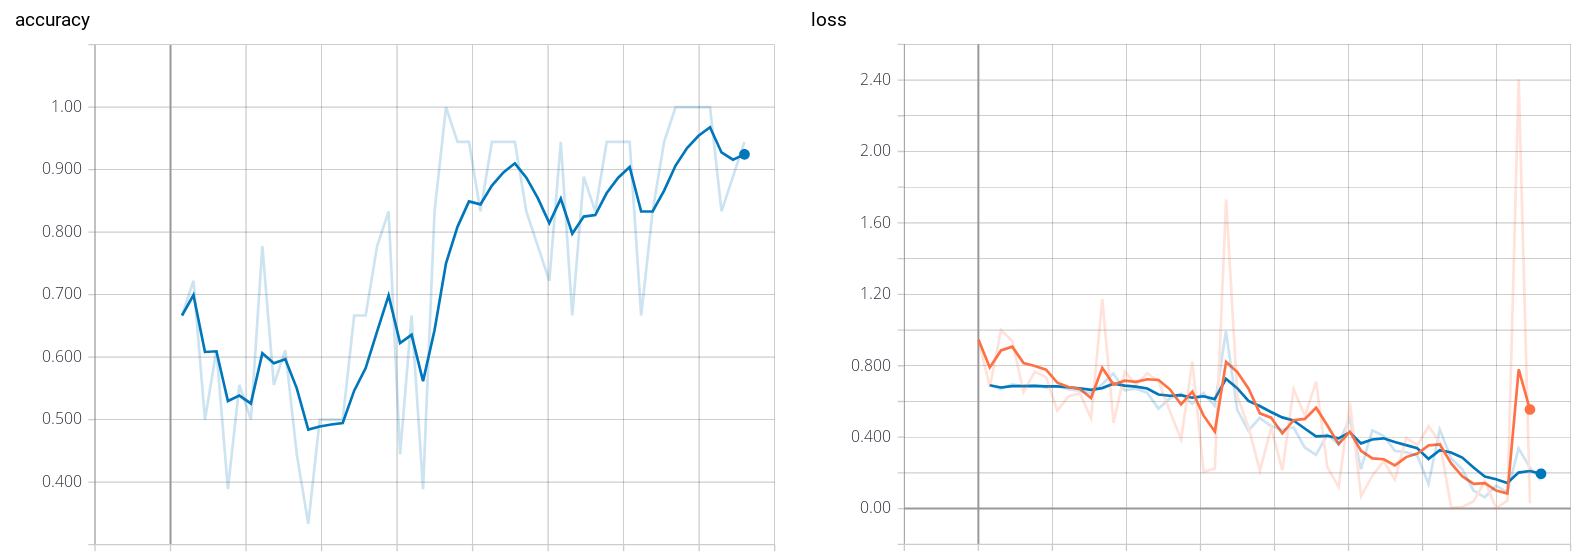
\includegraphics[width=\linewidth]{images/tests_7}
\caption{Experiment 7. Accuracy and loss of network for training and validation data.}
\label{fig:tests_7}
\end{figure}




\begin{table}
\caption{Test results for experiment 8.}
\resizebox{\linewidth}{!}{%
	\begin{tabular}{ | c | c | c | c | c | c | c | c | }
		\hline
		patient & $Y_i$ & $N_{hc}$ & $N_p$ & $C_{i,t} (\%)$ & $P_i$ & $\hat{Y}_i$ & $C_i (\%)$ \\  \hline
		CTL09 & HC & 102 & 96  & 51.51 &  0.5151 & HC  & 100 \\
		CTL12 & HC & 122 &  76  & 61.62 & 0.6162 & HC & 100 \\
		CTL06 & HC & 198 &   0  &  100   &    1       & HC & 100 \\
		ODP09 & P  &   0   & 198 &  100   &    0       &  P  & 100 \\
		ODP12 &  P  &   2   & 196 & 98.99 & 0.0101 &  P  & 100 \\
		ODP06 & P  &   0   & 198 &  100   &    0       &  P  & 100 \\ \hline
		\multicolumn{4}{|r|}{$\overline{C_{i,t}}$} & 85.35 &
		\multicolumn{2}{|r|}{$\overline{C_{i}}$} & 100 \\
		\hline \hline
		
		\multicolumn{2}{|r|}{True positive (TP)} & 
		\multicolumn{2}{c|}{ 3 } &
		\multicolumn{2}{|r|}{False positive (FP)} & 
		\multicolumn{2}{c|}{ 0 } \\ 
		\multicolumn{2}{|r|}{False negative (FN)} & 
		\multicolumn{2}{c|}{ 0 } &
		\multicolumn{2}{|r|}{True negative (TN)} & 
		\multicolumn{2}{c|}{ 3 }  \\
		\hline \hline
		
		\multicolumn{2}{|r|}{Time-slice TP} & 
		\multicolumn{2}{c|}{ 422 } &
		\multicolumn{2}{|r|}{Time-slice FP} & 
		\multicolumn{2}{c|}{ 2 } \\ 
		\multicolumn{2}{|r|}{Time-slice FN} & 
		\multicolumn{2}{c|}{ 172 } &
		\multicolumn{2}{|r|}{Time-slice TN} & 
		\multicolumn{2}{c|}{ 592 }  \\
		\hline \hline
		
		\multicolumn{2}{|r|}{Time-slice sensitivity} & 
		\multicolumn{2}{c|}{ 0.71043771 } &
		\multicolumn{2}{|r|}{Sensitivity} & 
		\multicolumn{2}{c|}{ 1 } \\ 
		
		\multicolumn{2}{|r|}{Time-slice specificity} & 
		\multicolumn{2}{c|}{ 0.996632997 } &
		\multicolumn{2}{|r|}{Specificity} & 
		\multicolumn{2}{c|}{ 1 } \\ 
		
		\multicolumn{2}{|r|}{Time-slice PPV} & 
		\multicolumn{2}{c|}{ 0.995283019 } &
		\multicolumn{2}{|r|}{PPV} & 
		\multicolumn{2}{c|}{ 1 } \\ 
		
		\multicolumn{2}{|r|}{Time-slice NPV} & 
		\multicolumn{2}{c|}{ 0.77486911 } &
		\multicolumn{2}{|r|}{NPV} & 
		\multicolumn{2}{c|}{ 1 } \\ \hline
	\end{tabular}
}
\label{table:tests_8}
\end{table}
\begin{figure}
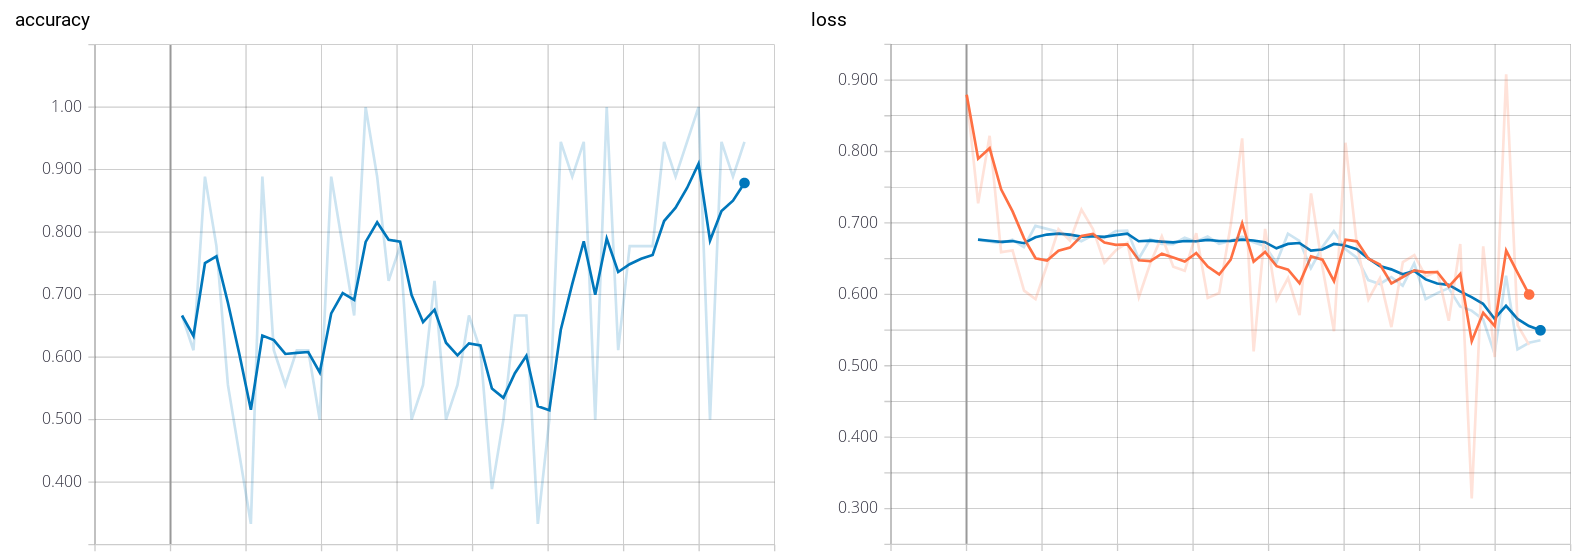
\includegraphics[width=\linewidth]{images/tests_8}
\caption{Experiment 8. Accuracy and loss of network for training and validation data.}
\label{fig:tests_8}
\end{figure}













\section{Discussion}
\label{section:discussion}



















\begin{figure}
	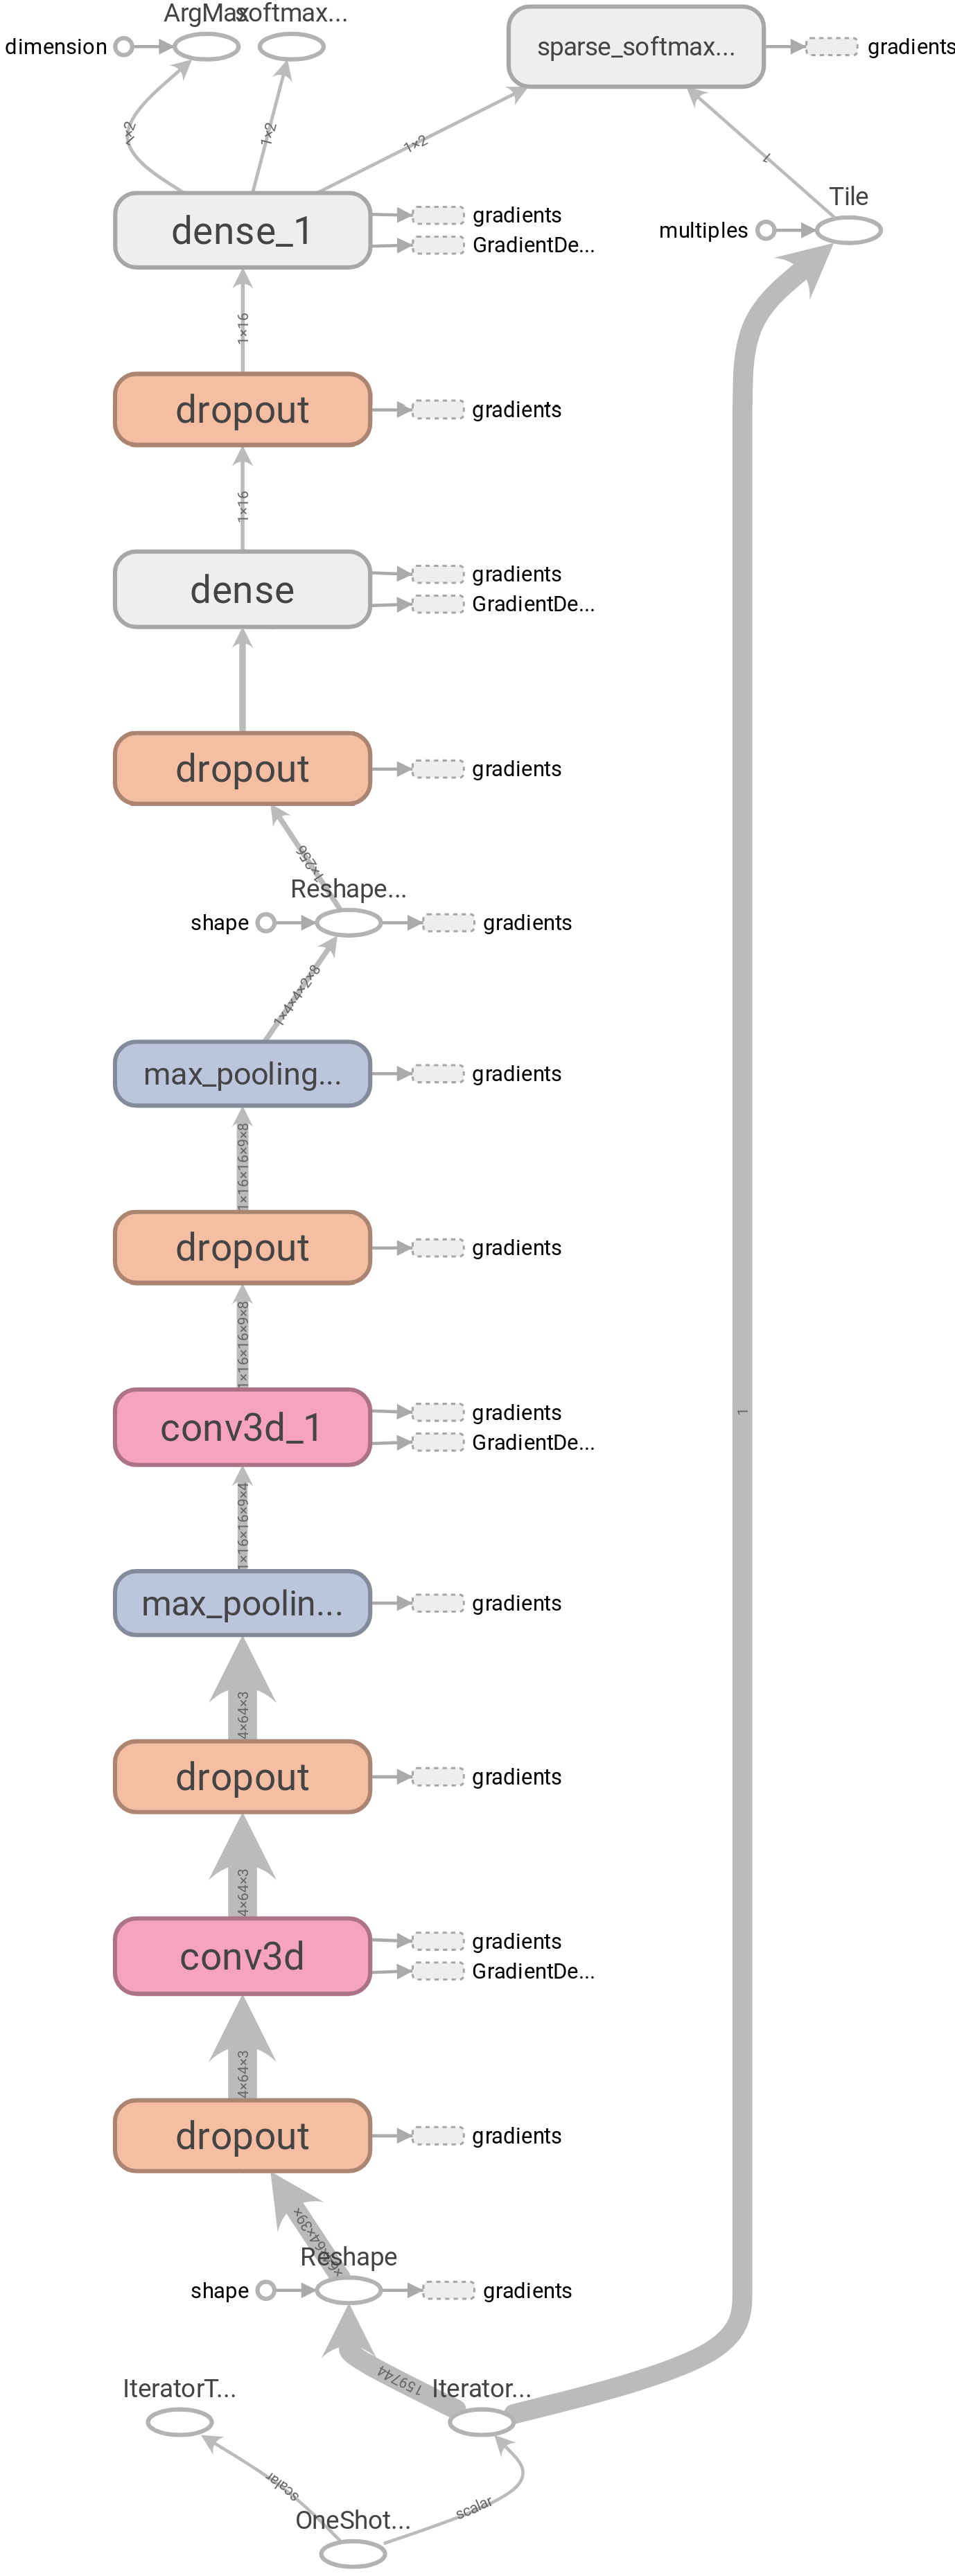
\includegraphics[width=\linewidth]{images/cnnArch}
	\caption{Proposed Bayesian 3D CNN architecture}
	\label{fig:cnnArch}
\end{figure}

\appendix
\section{My Appendix}
Appendix sections are coded under \verb+\appendix+.

\verb+\printcredits+ command is used after appendix sections to list 
author credit taxonomy contribution roles tagged using \verb+\credit+ 
in frontmatter.

\printcredits

%% Loading bibliography style file
%\bibliographystyle{model1-num-names}
\bibliographystyle{cas-model2-names}

% Loading bibliography database
\bibliography{refs}


%\vskip3pt


\end{document}

